%BEGIN_FOLD
%----------------------------------------------------------------------------------------
%   PACKAGES AND OTHER DOCUMENT CONFIGURATIONS
%----------------------------------------------------------------------------------------

\documentclass[12pt, a4paper, twocolumn, fullpage]{article}
\usepackage{algorithm}
\usepackage{color}
\usepackage{graphicx}
\usepackage{amssymb}
\usepackage{amsthm}
\usepackage{lipsum}
\usepackage{algorithmic}
%\usepackage[round]{natbib} TODO in future
\usepackage{titlesec}
\titleformat*{\section}{\Large\bfseries}
\titleformat*{\subsection}{\large\bfseries}

\usepackage{amsmath,amsfonts,amssymb,amsthm,epsfig,epstopdf,titling,url,array}


\theoremstyle{plain}
\newtheorem{thm}{Theorem}[section]
\newtheorem{lem}[thm]{Lemma}
\newtheorem{prop}[thm]{Proposition}
\newtheorem*{cor}{Corollary}

\theoremstyle{definition}
\newtheorem{defn}{Definition}[section]
\newtheorem{conj}{Conjecture}[section]
\newtheorem{exmp}{Example}[section]

\theoremstyle{remark}
\newtheorem*{rem}{Remark}
\newtheorem*{note}{Note}

%---------
%   ARTICLE INFORMATION
%----------------
\title{Topological Classification of SCOPe}
\author{Yechan Hong, Jan Segert, and Jianlin Cheng
\and University of Missouri, Columbia}
\date{\today}
%END_FOLD
\begin{document}
\maketitle

% ====================================
\section*{Abstract}
% ====================================

\textbf{Motivation:} SCOPe 2.07 is a database of 276,231 protein domains that have been partitioned into varying folds according to their shape and function. Since a protein's fold reveals valuable information about it's shape and function, it is important to find a mapping between protein's and it's fold. There are existing techniques to map a protein's sequence into a fold \cite{deepsf} but none to map a protein's shape into a fold. We focus on the topological features of a protein to map it into a fold. We introduce several new techniques that accomplish this.
\\
\textbf{Results:} We develop a 2D-convolutional neural network to classify any protein structure into one of 1232 folds. 
We extract two classes of input features for each protein's carbon alpha backbone: distance matrix and the persistent homology barcodes. Due to restrictions in our computing resources, we make sample every other point in the carbon alpha chain. We find that it does not lead to significant loss in accuracy.
Using the distance matrix, we achieve an accuracy of 86\% on the entire dataset.

We extract significant topological simplices of the protein by using persistent homology. We format the persistent homology data into various input features: persistence images \cite{persistenceImages}, simplex distance map, and simplex grouping.  With persistence images of 100x100 resolution, we achieve an accuracy of 62\% on SCOP 1.55. With simplex distance maps of 100x100 resolution, we achieve an accuracy of 70\%. With simplex groupings, we achieve an accuracy of :TODO\%.
    
%   We also combine the different classes of input features to achieve an accuracy of :TODO\%. An analysis on the network is performed to qualitatively describe the features the network is using to accurately classify the proteins.

% ====================================
\section{Introduction}
% ====================================
    Add introduction in literature and background information here. Future work to be added here. Discussion of topological data analysis will also be added here.

% ====================================
\section{Material}
%====================================

%----------------------
\subsection{Datasets}
%----------------------

The SCOP database is a database of proteins organized into hierarchical classes based on their shape and function. There are 4 levels of the hierarchy (top down): Class, Folds, Superfamily, Family. We will be primarily concerned with the Fold.

Two different versions of the dataset were used, SCOP 1.55 and SCOPe 2.07. SCOP 1.55 is a smaller dataset which is a subset of SCOPe 2.07, a larger and more recent dataset. SCOP 1.55 [Ref: Biblio] and SCOPe 2.07 [Ref: Biblio] were downloaded from the Berkeley repository as tar files and unpacked. For each of the datasets, index files [Ref:Biblo] are provided.

\subsubsection{Small Dataset SCOP 1.55}

SCOP 1.55 is a dataset of 31,474 proteins that have been organized into 7 Classes, 605 Folds, 947 Superfamilies, and 1557 Families. The dataset was released and updated till 2001. This dataset is a subset of the SCOPe 2.07 dataset.


\begin{figure}[t]
    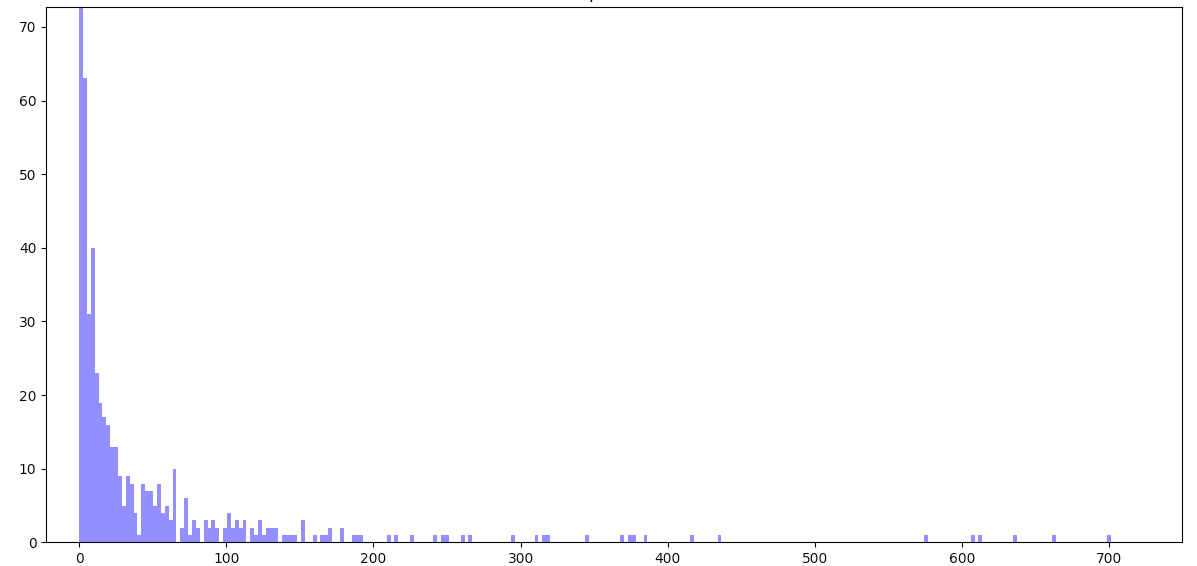
\includegraphics[width=\linewidth]{num_proteins_fold_155}
    \caption{Here is a histogram of the number of proteins per fold for SCOP 1.55. We see that most of the folds do not have too many proteins. This could be a potential issue during learning.}
    \label{num_proteins_fold_155}
\end{figure}

We inspect the distribution of the proteins across the different folds. We see that most of the folds do not have a lot of proteins. The median number of proteins per fold was 10 and the histogram (Fig.\ref{num_proteins_fold_155}) show that most of our proteins have less than 50 proteins per fold. This would likely impact our learning, since there are not too many examples for the protein to learn.


\begin{figure}[t]
    \includegraphics[width=\linewidth]{chainlengths155}
    \caption{Here is a histogram of the protein lengths for SCOP 1.55. We see that 90\% of the proteins have length less than 500}
    \label{chainlengths155}
\end{figure}

We also inspect the size of the proteins in our database (Fig. \ref{chainlengths155}). We define the size of the protein to be the length of the protein (Background Information: Proteins Information). We see that most of the proteins have length less than 300. We do see a small amount of our proteins having lengths between 600 to 800. 

We split up 70\% of the dataset for training, 15\% for validation and 15\% for testing. We adjust the sampling of the validation and testing so that a wide range of folds are represented.

New methods were tested on the small dataset. This allowed us to quickly prototype and optimize our methods to run on the larger dataset.

\subsubsection{Large Dataset SCOPe 2.07}

SCOPe 2.07 is a database of 276,231 proteins that have been organized into 7 Classes, 1232 Folds, 2026 Superfamilies, and 4919 Families. The dataset was released and updated till 2017. This dataset contains and is about 9 times larger than the SCOP 1.55 dataset.

\begin{figure}[t]
    
\includegraphics[width=\linewidth]{img/blank.png}
    \caption{Here is a histogram of the number of proteins per fold for SCOP 2.07. We see that each fold has much more examples than SCOP 1.55. This may allow our model to learn better.}
    \label{numproteinfold2.07}
\end{figure}

We inspect the distribution of the proteins across the different folds. We see that there are much more proteins per fold.

\begin{figure}[t]
    
\includegraphics[width=\linewidth]{img/blank.png}
    \caption{Here is a histogram of the protein lengths for SCOP 2.07. We see that 90\% of the proteins have length less than 500}
    \label{chainlength2.07}
\end{figure}

Once again, we inspect the size of the proteins in our dataset.

Similar to the small dataset, we split up 70\% of the dataset for training, 15\% for validation and 15\% for testing. We adjust the sampling of the validation and testing so that a wide range of folds are represented.
    
\subsection{Third Party Tools}

A number of third party tools were used as part of the research. ProDy's (Protein Dynamics \& Sequence Analysis) python package was used to extract the backbone structure from each protein's PDB file. NumPy package was used for matrix  and statistical operations. Matplotlib package was used to generate histograms and 3D plots of the proteins and the barcodes. Pillow was used to generate the 2D images of the distance matrix and the barcode images. Keras and Tensorflow were used to setup and train the convolutional neural network. CPickle package was used to serialize and deserialize processed data.
    
\subsection{Computing Resources}

Initially the research started on a personal laptop without a GPU and very limited storage space [Ref: Table]. Since the unpacked data of SCOPe 2.07 took up around 40GB and the laptop ran out of storage space, the data was stored on a flash drive. 

The lack of a GPU made the training very slow. Even relatively simple methods on the smaller, SCOP 1.55, dataset took around 40 hours. Furthermore, the small storage space made it difficult to unpack and save the processed data on the larger SCOPe 2.07 dataset. These factors significantly slowed the progress of the research.


\begin{table}[t]
    \centering
    \begin{tabular}{c | c}
        CPU & Intel Core i7-4650U \\ \hline
        GPU (CUDA-enabled) & None     \\ \hline
        RAM & 8GB    \\ \hline
        Storage & 128GB SSD \\ \hline
        OS & MacOSx  
    \end{tabular}
    \caption{Personal Latop}
    \label{tbl:Computer 1}
\end{table}

Due to the limitations of the personal laptop, a personal workstation was purchased at \$500 on Winter of 2018 [Ref: Table]. Although it has modest computing power relative to industry standards, the purchased machine led to significant increases in speed and efficiency of the research. The most important changes in computer resources were the GPU, which led to increases in training speed, and the increased storage, which made it possible to work on the larger SCOPe 2.07 dataset. It is also worth nothing that Ubuntu has better support than MacOSx for running CUDA.
Most of the optimized methods took around 16 hours at most to complete on the large SCOPe 2.07 database, which is 8 times larger than the smaller SCOP 1.55. 

\begin{table}[t]
    \centering
    \begin{tabular}{c | c}
        CPU & E5-2630 6-Core \\ \hline
        GPU (CUDA-enabled) & Nvidia GTX 1060 6GB     \\ \hline
        RAM & 16GB    \\ \hline
        Storage & 500GB SSD \\ \hline
        OS & Ubuntu 16.02  
    \end{tabular}
    \caption{Personal Workstation}
    \label{tbl:Computer 2}
\end{table}

% ===============================================================
\section{Methods}
% ===============================================================

%---------------------
\subsection{ Background Information: Proteins} \label{Background Information: Proteins}
%---------------------
A protein is an sequence of amino acids, 2 compounds which link into a protein chain. The interaction between amino acids and the surrounding environment determine the how the protein folds into its structure.

For a protein that we are tasked to classify, we are provided with many information: Protein sequence and the sequential coordinates of every atom on our protein. Since we are primarily interested in the topological features of our data, we characterize the protein's shape with the protein backbone. The protein's backbone is constructed with a sequence of points, where each point represents each amino acid in a 3D space. The point representation of each amino acid is determined by the algorithm 'parsePDB' in the ProDy package. 

Since we will be dealing primarily with the protein's backbone, we introduce the following notation.
    
\begin{defn}
A protein, $P$, with sequence of N amino acids will be a called a protein with length N. It's backbone will be denoted as a sequence of 3D coordinate points $ \{P_i\}^{N}_{i=1} $ where $P_{i} \in \mathbb{R}^3 $

For each coordinate point $ P_{i} $, the x-coordinate is referred as $ P_{i}(1) $, y-coordinate as $ P_{i}(2) $, and z-coordinate as $ P_{i}(3) $.
\end{defn}

We extract two distinguishing types of input features from the protein's backbone chain: Distance matrix and Persistence Homology. These two features are very robust. They are both rotation and translation invariant, meaning that the features remain the same even if the protein is rotated or moved. They are also very stable: minor changes to the data does not create a significant variation in the feature.
    
%---------------------
\subsection{ Backbone Chain}
%---------------------  
Each the dataset of proteins are stored as PDB (Protein Data Bank) files, which describe the shape of the 3D protein. The dataset tar [Ref] files unpack into main directory, pdbstyle-1.55 and pdbstyle-2.07 for SCOP 1.55 and SCOPe 2.07 respectively. Each PDB file is stored in a subdirectory under the main directory. The name of the subdirectory is determined by the protein's name.

The index files for SCOP 1.55 and SCOPe 2.07, 'dir.cla.scop.1.55.txt' and 'dir.cla.scope.2.07-stable.txt', provide important information for each protein in our database [Ref: index example]. 

\begin{table}[t]
    \centering
    \begin{tabular}{c | c}
        Index Line & d1dlwa\_ 1dlw    A:  a.1.1.1 ... \\
        Name & d1dlwa\_     \\
        Class.Folds.Superfamily.Family & a.1.1.1    \\
    \end{tabular}
    \caption{Index Entry. The PDB file for this protein found under the subdirectory 'dl' as 'd1dlwa\_.ent'}
    \label{tbl:Index Entry}
\end{table}

For each protein, protein backbone chain is parsed from the PDB file using the 'parsePDB' function in the ProDy package. The extracted coordinates of the protein backbone is saved as a list. 

The class and the fold number of the protein uniquely identifies a protein's fold. We create a one to one mapping between class-fold to the integers. These integers are the labels of our protein-fold classification problem.

Because all of the protein coordinates do not fit on the RAM, they are saved in batches of 10000. In each batch, the protein coordinates and the fold labels are saved into a dictionary under the keys b'x' and b'y' respectively.

%---------------------
\subsection{ Distance Matrix}
%---------------------
With the points in the protein backbone, we construct a distance matrix of the distances between the points. The unit of the distances Ångströms, the units of provided in the protein PDB files. [Protein Data Bank]. We used the Euclidean Distance for the distances between the points.

    
\begin{defn}
    For a protein $P$ with length N, we denote it's distance as matrix $M_{P}$.
    We construct it as follows.
    $ M_{P} := [M_{ij}] $ where 
    \begin{multline*}
    M_{ij} = Euclidean Distance(P_i, P_j) = \\ \sqrt{P_i(1)-P_j(1))^2+(P_i(2)-P_j(2))^2} \\ +(P_i(3)-P_j(3))^2
    \end{multline*}
\end{defn}

\noindent
\textbf{Remark}
\\
    We note the following for any distance matrix $M_{P}$.
    \begin{itemize}
        \item $M_{ii} = 0$
        \item $M_{ij} = M_{ji}$
        \item The intersection of the ith row and the jth column corresponds to $M_{ij}$, the distance between the ith and the jth point.
    \end{itemize}
    
\begin{figure}[h]
    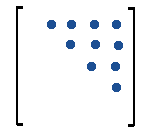
\includegraphics[width=\linewidth]{uptry.png}
    \caption{Here we have the entries in a matrix that correspond to the upper triangle. We note that since our distance matrix is symmetric with respect the diagonal line, we only need to calculate the distance values once for the entries in the upper triangle of our matrix.}
     \ref{uptry}
    \label{uptry}
\end{figure}
    

We see that the distance matrix is symmetric (Fig.\ref{uptry}) since the distance between the ith and the jth point is the same as the distance between the jth point and the ith point. Because of this, we only need to compute the distance between these pairs of points once. Also, the distance between a point to itself is zero. So the pairs of ith and jth's points we need to compute the distances for lie in the upper triangular region of the distance matrix. This region is consists of $\{ M_{ij} \space | \space i<j \}$ [Ref:]. Computing the distance matrix in this fashion divides the computation time by about half. Because the distance matrices of the entire dataset are larger than the size of the RAM, the data is split up into 1000 sized batches. 

\begin{algorithm}
\caption{We fill in our distance matrix by calculating the upper triangle of a NxN matrix. Our rows and columns range from 1 to N.}
\begin{algorithmic}
\STATE{M is distance matrix set with zeroes}
\STATE{Euclid(a,b) is the distance between a and b}
\FOR{r <= N}
    \FOR{c < r}
    	\STATE{d=Euclid(r,c)}
        \STATE{M(r,c)=d}
        \STATE{M(c,r)=d}
    \ENDFOR
\ENDFOR
\end{algorithmic}
\end{algorithm}

\begin{figure}[h]
    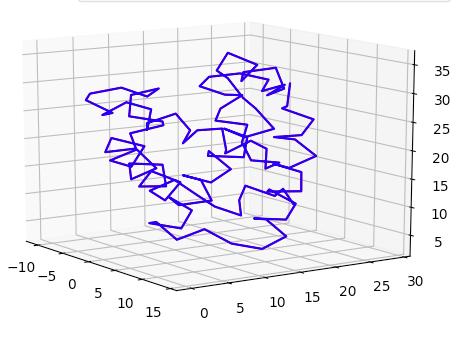
\includegraphics[width=\linewidth]{1ux8pdb.png}
    \caption{Here is the 3D shape of the  1ux8 protein's backbone chain. We see that there are notable features, alpha helices and beta sheets, that we would like to represent in our distance matrix.}
    \label{1ux8pdb}
\end{figure}

We inspect the topological structure of our protein '1ux8'. It is a protein of length 118. This protein has some spiral structures (alpha helix). These spiral structures sometimes lie in close promixity in parallel or anti parallel direction (beta sheet). These types of structures (secondary structures) are known in molecular biology to be important features of a protein's shape.

\begin{figure}[h]
    \centering
    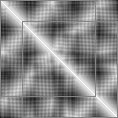
\includegraphics[width=.7\linewidth]{1ux8matBase}
    \caption{Here is the distance matrix of the 1ux8 protein. We see a thick diagonal line with corresponds to the protein backbone chain.}
    \label{1ux8matBase}
\end{figure}
    
We analyze the distance matrix to see if important structural features are represented in the matrix. To help with visualization, the distance matrix is mapped to an image of equal size, where closest distances appear in white and furthest distances appear in black. Distances in between take a gray hue with the intensity based on its value.
\\
\noindent
\textbf{Feature Protein Backbone:}
Along the diagonal line of the image, the distance matrix is completely white. This is because the distance between a point to itself is zero [Ref: Remark]. We note that this diagonal white line uniquely identifies the protein backbone chain (Since the distance between. Having a clear representation of the protein backbone is important because  it is a central structure that other features can be spatially oriented around.
\\
\noindent
\textbf{Feature Alpha Helix:}
We note thick white regions running parallel along the diagonal line of the image [Ref: Image]. These regions indicate that at a given point in the chain, it is in close proximity to the nearby neighbors [Ref Diagram]. We also note that in for a point in an Alpha Helix, it is also in close proximity to it's nearby neighbors. In our example, these four thick white regions correspond the the four helix structures on our protein.
    
\begin{figure}[h]
    \centering
    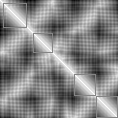
\includegraphics[width=.7\linewidth]{1ux8matAhelix}
    \caption{The red squares outline the discrete thick white regions running parrallel to the diagonal line. These regions indicate that the neighbors of points in this region are in very close proximity, indicating that there may be a helix. }
    \label{1ux8matAhelix}
\end{figure}

    
\begin{figure}[h]
    \centering
    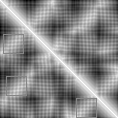
\includegraphics[width=.7\linewidth]{1ux8matBetaSheets}
    \caption{The green squares outline the lines of proximity between points on different helicies, suggesting that the helices are in close proximity. The direction of the lines indicate whether the two helices are parallel or anti-parallel.}
    \label{1ux8matBetaSheets}
\end{figure}

\begin{defn}
A helix is composed of points in the protein backbone. Suppose $H$ is the set of indices of these points along the length of the protein. We call the row belonging to this helix as the collection of rows, $R_{i}$, of the distance matrix such that the rows contain elements of the helix. $\{R_{i} \space | \space i \in H \}$. Similarly we define the column belonging to the helix as $\{C_{i} \space | \space i \in H \}$.
\end{defn}

\noindent
\textbf{Feature Beta Sheet:}
We note patches of thick white lines in the intersection of the rows belonging to a helix and the columns belonging to another helix [Ref Diagram]. This indicates that the points of the two helices, and hence the two helices, are in close proximity. In particular, the regions are close sequentially: the ith point in helix A is close to the jth point in helix B and the i+1 th point in helix A is close to the j-1 th point in helix B. This sequential relationship describes a Anti-parallel Beta Sheets. For Parallel Beta Sheets, the i+1 th point would be close to the j+1 th point. In our example, the 3 pairs of Beta-sheets formed the 4 helices are represented in our distance matrix.
    
\subsection{ Cropped Distance Matrix}

Some proteins have a length of 600, making the distance matrix have a size of 600x600. However, due limitations on the GPU memory, it is not possible to construct a convolutional network with our input being 600x600. We would also like to crop the distance matrix such that the central backbone of the protein runs through the diagonal of our matrix. To crop and preserve the diagonal protein backbone, we take a 100x100 window and crop our matrix by shifting row and columns at the same time by 50 indices.

\begin{figure}[h]
    \centering
    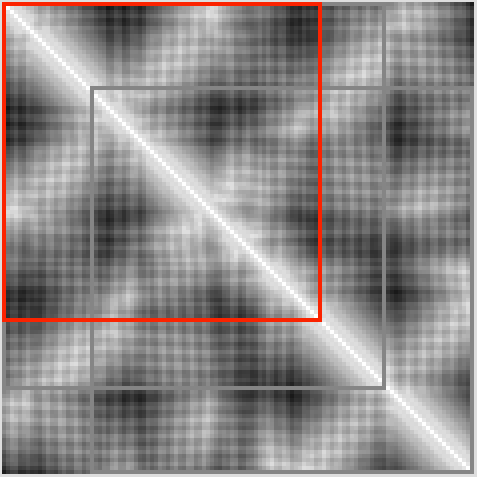
\includegraphics[width=.7\linewidth]{cropMat}
    \caption{Due to computational restrictions, we crop our matrix by shifting the red crop window along the diagonal line of our matrix.}
    \label{cropMat}
\end{figure}

Because of the limitations set by the windowed distance matrix, a point in the backbone can only see information about, on average, half of the window size forwards and backwards. This limitation affects the cropped matrix's ability to detect longer range contact information, which can be critical in determining the protein's overall shape. In our example [Ref], the cropped distance matrix would not see information about the proximity between the first alpha helix and the third alpha helix because they are too far away in the backbone index.

\begin{figure}[h]
    \centering
    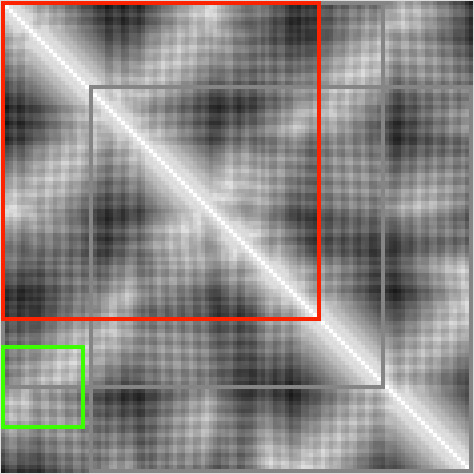
\includegraphics[width=\linewidth]{cropMatMiss}
    \caption{We note that cropping the distance matrix may cause a loss of long range contact information. In our protein 1ux8, the cropped matrices do not detect that the alpha helix 1 forms a beta sheet with alpha helix 3}
    \label{cropMatMiss}
\end{figure}

We note that if a distance matrix is smaller than our cropping window size, we pad the distance matrix.

Cropping the dataset increases the number of examples in the dataset. Because we don't want our training data to have similarities, we make sure that the training, validation, and testing groups do not share cropped matrices from the same protein.

\subsection{ Sparse Distance Matrix}

In our example, we see that cropping the distance matrix diminishes it's ability to represent long range contact information. We develop an alternative approach to reduce the size of the distance matrix while preserving it's ability to represent long range contact information.

\begin{figure}[h]
    \centering
    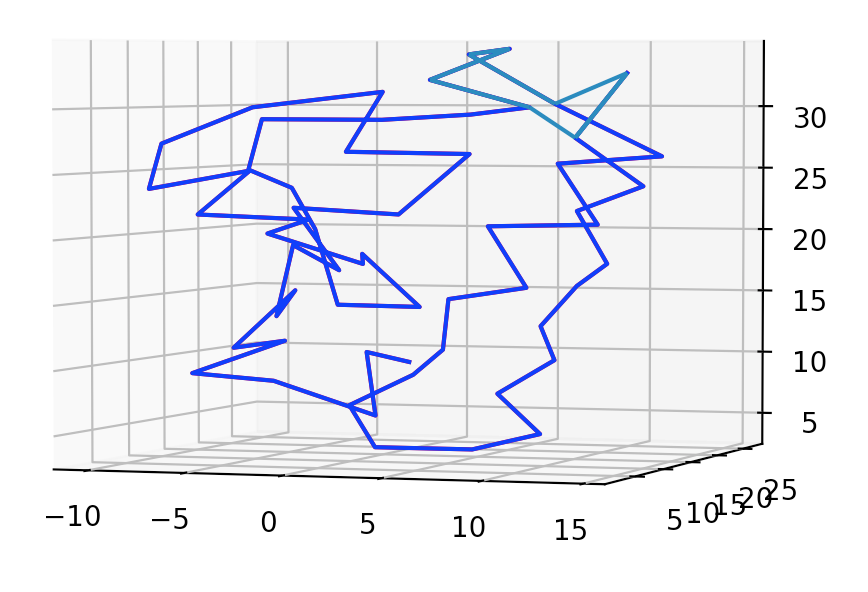
\includegraphics[width=\linewidth]{1ux8sparse}
    \caption{Due to computation restrictions, we sample every other point on our protein and compare it with the original structure. We see that, although diminished, most of the features of the protein are still distinguishable.}
    \label{1ux8sparse}
\end{figure}

Given, a protein backbone with length N, $\{P_i\}^{N}_{i=1}$, we sample every other point, $\{P_i \space | \space \text{i is odd} \}$, to create a sparse protein backbone. We graph the sparse protein backbone in 3D space [Ref ] and compare it to the original protein backbone [Ref: Original Chain]. In comparison, we see that the general structure of the protein and its features are diminished but preserved.

\begin{figure}[h]
    \centering
    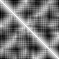
\includegraphics[width=.7\linewidth]{1ux8pdbSparseDistM}
    \caption{Here we have a distance matrix of the sampled 1ux8 protein backbone. We do see that the protein backbone, alpha helices, and beta sheets that were observed in the full distance matrix can also be observed in the sparse distance matrix. }
    \label{1ux8pdbSparseDistM}
\end{figure}

From the sparse protein backbone, we construct a sparse distance matrix in the same fashion as a regular distance matrix. In example, we compare the sparse distance matrix [Ref:] and the unmodified distance matrix [Ref:] and see if the backbone chain, alpha helix and beta sheet features are preserved in the distance matrix. First, we see that the diagonal backbone is preserved in the matrix. Second, we do see that the alpha helix features are preserved, even though it is less clearly defined. Finally, we see that the beta sheet features are preserved as well.

For the protein of length 600, the sparse distance matrix would reduce the matrix's size from 600x600 to 300x300. This is still too big for due to the limitations on the GPU memory. So we crop the sparse distance matrix in the same manner as a regular distance matrix. We also take care such that the training, validation, and testing groups do not share cropped matrices from the same protein.

%----------------------
\subsection{Convolutional Network Model}
%----------------------

The features from each of these subsections were fed into a a 2D-convolutional network. The architecture of the 2D-convolutional network for mapping protein structure to folds contains, in order, 32 3x3 convolutional layers, 64 3x3 convolutional layers, 2x2 max pooling, 128 dense layer, and the output layer.

\begin{figure}
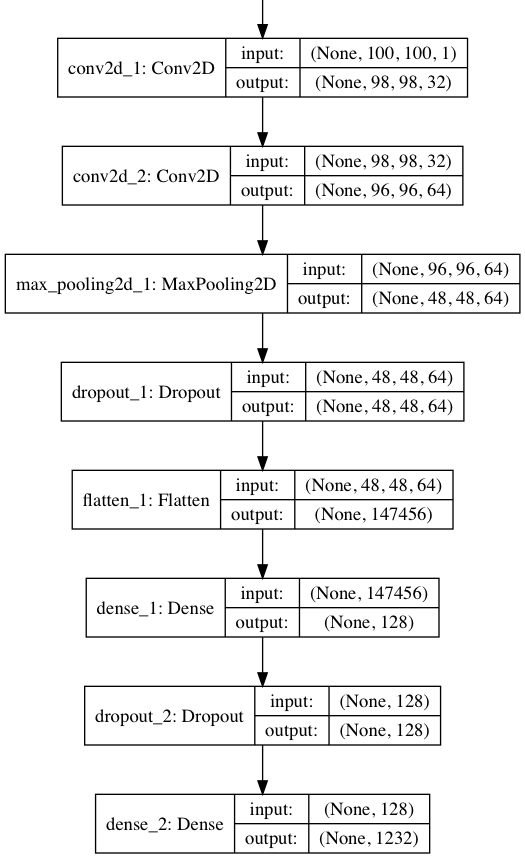
\includegraphics[width=\linewidth]{model_plot.png}
\caption{The architecture of a 2D deep convolutional network for protein fold classification. Convolutional layers were added as part of a traditional image classification network. Dense layers were added to help the network use the discovered features in the images. A dropout layer was added to make our network learn an ensemble of different models}
\label{model_plot}
\end{figure}

This is a relatively simple network. However, for our task of classifying quarter million of proteins, it performs exceptionally well. 
\\
There are a lot of benefits for a simple network performing well. First, it ensures that the model is not overfitting the data. Second, it is much more feasible to inspect the network to understand how it is learning.


%---------------------
\subsection{ Persistent Homology}
%---------------------
\textbf{Persistent Homology: } Topological data analysis is applied to the points in the protein backbone to produce persistent barcodes. The barcodes indicate when simplexes are formed and are destroyed. Significant topological features of the data are represented by these barcodes.


\subsubsection{ Mathematical Background}

We discuss the mathematical theory behind persistent homology prior to introducing an algorithm to compute it.  First, we describe the elementary mathematical objects. Then we describe the topological features of a data that we want to extract using the structure theorem. We also discuss the stability of the topological features described by the stability theorem.

\begin{figure}[t]
\centering
    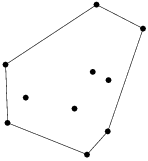
\includegraphics[width=.6\linewidth]{img/mathDef/ConvexHull2D}
    \caption{Illustration of a convex hull of 10 points. For a finite set of points this is just a a polygon connecting the outer most points.}
    \label{ConvexHull}
\end{figure}

\begin{defn}
A convex set, $C \subset \mathbb{R}^n$, is a set where $\forall a,b \in C, t \in [0,1] ta+(1-t)b \in C$. [Ref: Sakai]
\end{defn}

\begin{defn}
A convex hull $<A>$ of a set of points, $A \subset \mathbb{R}^n$ is defined by 
$$<A> := \bigcap \{C \mid C \text{ convex in } \mathbb{R}^n \text{ , } A\subset C \} $$
[Ref: Sakai]
\end{defn}

\begin{figure}[t]
    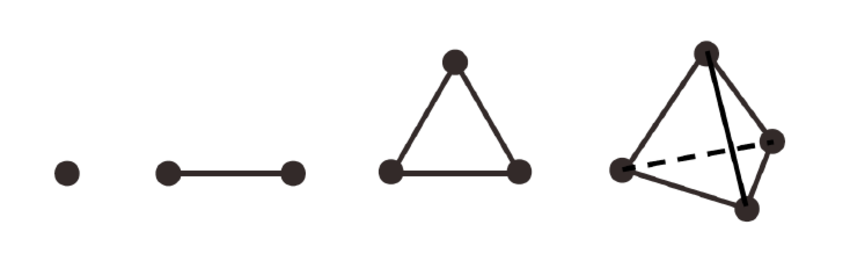
\includegraphics[width=\linewidth]{img/mathDef/simplex.png}
    \caption{Here are illustrations of a 0-Simplex (a point), 1-Simplex (a line), 2-Simplex (a triangle), 3-Simplex (a tetrahedron)}
    \label{Simplex}
\end{figure}

\begin{defn}
An n-simplex is a convex hull of n points. When we refer to varying sizes n-simplices or when the size is not determined, we will call them just simplices.
\end{defn}

\begin{defn}
Let $\sigma$ be a simplex.
The vertices of $\sigma$ are its points.
The face of $\sigma$ are the simplices formed by subset of the vertices of $\sigma$.
A n-face is a face of $\sigma$ with $n+1$ vertices.
\end{defn}

\begin{defn}
Simplicial complex is a set of simplices, $S $, such that 
\begin{itemize}
    \item Any face of a simplex $\sigma \in S$ is in $S$.
    \item The intersection of any two simplices in $ S $ is in $ S $
\end{itemize}
\end{defn}

\begin{figure}[t]
    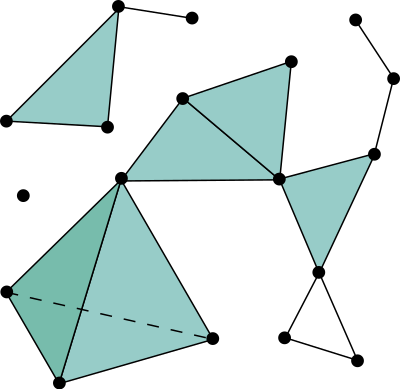
\includegraphics[width=\linewidth]{img/mathDef/simpcomplex}
    \caption{Here is an illustration of a simplicial complex. Notice that it is a collection of points,edges and triangles.}
    \label{simpcomplex}
\end{figure}

Now that we have defined the foundational definitions, we begin to define structures relevant to our problem of extracting topological features from our set of points in the protein backbone. First, we will observe the state of our data as we create triangular simplices from the points in our data by adding edges of increasing length. We do this by forming Vietoris-Rips complexes.

\begin{defn}
Given a set of points with a metric, a $\epsilon$-Vietoris-Rips complex is a simplicial complex which is formed on the set of points  by connecting the points with distance less than or equal to $\epsilon$
\end{defn}

\begin{figure}[t]
    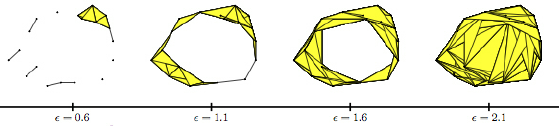
\includegraphics[width=\linewidth]{img/mathDef/ripscomplex.png}
    \caption{Here is a series of 5 Vietoris-Rips complexes. At $\epsilon=0$ we only have a collection of points, while at $\epsilon=1.1$ we being to see an interesting characteristic of our data beginning to form. Finally, at $\epsilon=2.1$ we do not see much of a structure as most of the points become interconnected to each other. }
    \label{}
\end{figure}

We see how the state of our data changes as we add edges between points of increasing length by ordering the $\epsilon$-Vietoris-Rips complexes in increasing order of $\epsilon$. This ordering is a filtration on the set of all Vietoris-Rips complexes on our data. If $\epsilon_1 \leq \epsilon_2$ then $\epsilon_1$-Vietoris-Rips complex is contained in  $\epsilon_2$-Vietoris-Rips complex. This is because edges less than $\epsilon_1$ are also less than $\epsilon_2$ and thus are formed in  $\epsilon_2$-Vietoris-Rips complex.

\begin{defn}
Let $\mathbb{S}$ be a collection of sets such that $\forall A \in \mathbb{S}$, $\exists B \in \mathbb{S}$ such that $A \subseteq B$ or $B \subseteq A$. That is given an element in our collection, it is contained or contains another set in our collection. 
A filtration is an ordering on $S_i \in \mathbb{S}$ such that
$$S_1 \subseteq S_2 \subseteq S_3 \subseteq S_4 \subseteq ...$$.
\end{defn}
 
We transform our filtration of Vietoris-Rips complexes to corresponding filtration where each Vietrois-Rips complex is converted to an algebraic group that can detect holes in our simplicial complex. We say that we apply a 1-homology, $H_1$ to each simplicial complex in our filtration. We get a new filtration of the form,

$$ H_1(S_1) \subseteq H_1(S_2) \subseteq H_1(S_3) \subseteq H_1(S_4) \subseteq ...$$.

Let $S$ be our simplicial complex. We will first construct the elements that define the homology on S.
\begin{defn}
The group of $k$-Chain of $S$ is an abelian group of elements consisting of 
$$\sum z_i s_i $$ where $z_i \in \mathbb{Z}$ and $s_i$ is a $k$-simplex of S.
We call this group $C_k$
\end{defn}

\begin{defn}
The boundary operator $\partial_k : C_k \rightarrow C_{k-1}$ is a homeomorphism where
$$\partial (\sigma) := $$ %TODO df%
$$\partial_1 (ab) := b-a$$
$$\partial_2 (abc) := ab+bc-ac$$
\end{defn}

\begin{defn}
Given a simplicial complex, $S$, it's j-homology is the algebraic quotient group, $\dfrac{Z_j}{B_j}$.
We define $Z_j = Ker \partial _j$ and $B_j = Im \partial_j$.
We denote the j-homology of $S$ as $H_j(S)$
\end{defn}
 
%TODO Write peristent module and structure theorem%
%TODO Write stabilty bottleneck and weistrauss%

\subsubsection{Computation Algorithm}
We describe our implementation of the persistent homology, in addition to variations to the method to improve performance and collect more protein specific simplices. 
In practice, we will use the N points of a protein backbone in this algorithm but for illustrative purposes, we consider a simple collection of N points in the $\mathbb{R}^2$. (Fig.\ref{Collection of points}) Because we are looking at the distances between our points, the method performs exactly the same in $\mathbb{R}^3$ or with any collection of objects with a well defined metric.

\begin{figure}[t]
    
\includegraphics[width=\linewidth]{img/blank.png}
    \caption{Here is the collection of the N points we are considering in 2D. Although our protein is in 3D, the method is concerned with the distances between points, allowing in to work in a similar fashion as this example.}
    \label{Collection of points}
\end{figure}

\begin{defn}
We call the (i,j) edge the edge constructed by connecting the ith and the jth point in our set of N points.
\end{defn}

A distance matrix of the our points is calculated. We collect the upper triangular elements of the distance matrix to get the unique edges of our points (unique disregarding direction, making (i,j) edge equal to (j,i) edge). These edges are sorted by length.

\begin{figure}[t]
    
\includegraphics[width=\linewidth]{img/blank.png}
    \caption{Here is a distance matrix of our set of N points. We will only consider the edges in the upper triangular matrix, because the (i,j) edge represents the same line as the (j,i) edge}
    \label{Distance matrix of example}
\end{figure}

Consider a protein with length 300. The total number of edges for a protein of length 300 is $\sum_{n=1}^{299} n =44851$. The total number of triangular simplices formed by these edges $\binom{300}{3}=\dfrac{300!}{3!297!}=4455100$.  We see that the numbers of triangular simplices increase exponentially and very quickly, even for small structures. This demands a need to reduce the computation load.

A cutoff distance is determined, where we discard the edges that are larger than this value. A similar concept exists in bioinformatics, where a point of a protein are determined to be in contact with another point if their distance is within the contact distance (3 Å). The loss of information by discarding the edges larger than this value isn't an issue since because when we start considering larger edges, we start converging towards a structure where every point is connected to each other. As long as we set the cutoff distance at an appropriate value, we would still get the cycles of the protein that represent the characteristic features. Furthermore, setting of a cutoff distance has an added advantage that it filters out uninteresting cycles that are too large. We determined the cutoff distance at 6.5 Å, because we experimentally determined that 6.5 Å is an upper bound of the distances between two alpha helices. The distance between two alpha helices are less than 6.5  Å, we  consider the edges that link two alpha helices together, allowing use to extract features related to the beta sheets. Furthermore, the sequential distances between the backbone points, $P_i and P_{i+1}$, and the distances within the alpha helices are both less than 6.5, allowing use to extract features related to them as well.

For our set of N points, the cutoff distance is determined as $\dfrac{1}{6}$ of the longest length, which is ?. Below are the collection of points 

\begin{figure}[t]
    
\includegraphics[width=\linewidth]{img/blank.png}
    \caption{Here we see the effect of the cutoff distance on the triangular simplicies we form. When a cutoff distance is not set, all the edges are considered, forming triangular simplicies where every point is connected to each other. These simplices don't convey too much about the structure of our protein. When a cutoff distance is set properly, the important distances considered, making the simplices less convoluted and increasing computation time.}
    \label{Effect of cutoff}
\end{figure}

Once we have the edges that we are considering, we find the triangular simplicies formed by our edges. As we loop over the edges, we index the edges from 1 to N based on the endpoints of the edge (For an edge (2,4),   it is indexed as 2 and 4). Then, we check if each edge forms a triangular simplicies by looking at the indexed edges related to our edge. (For an edge (2,4), we look at the edges that have been index as 2 or 4 to see if we formed a 2-simplex). Because we are forming the triangular simplicies as we add increasing edges, triangular simplicies are ordered by when they are created. 

\begin{algorithm}
\caption{Finding triangular simplicies formed by the edges}
\begin{algorithmic}
\FOR{(i,j) in Edges}
    \FOR{edges indexed i and indexed j}
        \STATE{See if these edges form a triangular simplicies with (i,j)}
    \ENDFOR
    \STATE{Index (i,j) as i and j}
\ENDFOR
\end{algorithmic}
\end{algorithm}

Given a triangular simplex, we can compute when it was born by looking at it's edges. For example, a triangular simplex (1,2,3) has the edges (1,2), (1,3), and (3,1). Suppose the lengths of these edges were 3,5, and 7 respectively. Then the triangular simplex was formed at radius 7. 

\begin{figure}[t]
    
\includegraphics[width=\linewidth]{img/blank.png}
    \caption{The triangular simplices are discovered as we add edges. Because we are adding the edges in increasing order, the triangular simplices are discovered in the order of their birth.}
    \label{Simplex formation algorithm}
\end{figure}

From the edges and triangular simplices, we create two matrices, D1 and D2. Let M be the number of edges we are considering and L be the number of triangular simplices we are considering.

\begin{figure}[t]
    
\includegraphics[width=\linewidth]{img/blank.png}
    \caption{Here is a D2 matrix for the protein 1ux8. We notice that most of the matrix consists of zero elements. }
    \label{D2Mat}
\end{figure}


D1 is a  NxM matrix where the rows correspond to the backbone points and the columns corresponds to the edge in increasing order. We fill in D1 in the following order. For the hth  edge with endpoints (i,j), we set $D1_{h,i} = -1$ and $D1_{h,j} = 1$. Suppose an edge (2,4) is the 10th smallest edge. The corresponding entries in would be $D1_{10,2}=-1$ and $D1_{10,4}=1$.

\begin{algorithm}
\caption{Constructing D1}
\begin{algorithmic}
\FOR{hth edge (i,j) in Edges}
    \STATE{$D1_{h,i} = -1$}
    \STATE{$D1_{h,j} = 1$}
\ENDFOR
\end{algorithmic}
\end{algorithm}

D2 is a MxL matrix where the rows correspond the edges in increasing order and the columns correspond to the triangular simplicies in created order. We fill in D2 in the following order. For the hth triangular simplex with endpoint (i,j,k), we set $D2_{h,i} = 1$, $D2_{h,j} = 1$ , and $D2_{h,k} = -1$. Suppose an edge (2,4,9) is the 10th triangular simplex. The corresponding entries in would be $D2_{10,2}=1$, $D2_{10,4}=1$, and $D2_{10,9}=-1$. 

\begin{algorithm}
\caption{Constructing D2}
\begin{algorithmic}
\FOR{hth edge (i,j,k) in Edges}
    \STATE{$D2_{h,i} = 1$}
    \STATE{$D2_{h,j} = 1$}
     \STATE{$D2_{h,k} = -1$}
\ENDFOR
\end{algorithmic}
\end{algorithm}

Each of the matrices, D1 and D2, are reduced to echelon form with the following algorithm. A pivot at a given column is given by the last nonzero entry in the column. We try to make all the columns not share any pivots. We loop over the columns and set check if the previous columns share a pivot with the current column. If they share a pivot, a multiple of the sharing pivot is subtracted from the current pivot such that the they do not share pivots. This process is repeated until the current column does not share a pivot with any of the previous columns. Every time the matrix is modified the same operation is performed to an identity matrix, MxM identity matrix for D1 and LxL identity matrix for D2. After we finish reducing the matrix, we call the reduced matrix R1 and R2 and the corresponding modified identity matrices V1 and V2.

\begin{algorithm}
\caption{Reduction of a matrix}
\begin{algorithmic}
\FOR{column in Columns of D2}
    \FOR{pcolumn in Columns before column}
        \IF{column share the same pivot as pcolumn} 
            \STATE{k=$\dfrac{column[pivot]}{pcolumn[pivot]}$}
            \STATE{column -= k*pcolumn}
        \ENDIF
    \ENDFOR 
\ENDFOR
\end{algorithmic}
\end{algorithm}

Finally, we can construct the main matrix that gives us the persistence homology of our protein. First we construct matrix B from the nonzero columns of matrix R2.  Second we construct matrix Z from columns of V1 corresponding to zero columns of R1. The main matrix is then constructed by taking matrix B and appending columns from matrix Z which do not share pivots with columns of our main matrix until the total number of columns is equal to the number of columns in matrix Z.

\begin{algorithm}
\caption{Construction of Main Matrix}
\begin{algorithmic}
\STATE {Main = B}
\FOR{column in Columns of Z}
    \IF{number of columns in Main equals number of columns in Z}
        \STATE{Exit Loop}
    \ENDIF
    \IF{column doesn't share pivots with columns of Main}   
        \STATE{Append column to Main}
    \ENDIF
\ENDFOR
\end{algorithmic}
\end{algorithm}

\begin{figure}[t]
    
\includegraphics[width=\linewidth]{img/blank.png}
    \caption{Here we have a diagram of the matrices that we have constructed and manipulated. The final product, the main matrix, is a MxH matrix where M is the number of edges we have considered and H is the simplex with persistent homology.}
    \label{MatricesOfComputeHom}
\end{figure}

The columns in the main matrix which come from B correspond to the simplices which get created and filled in before our cutoff distance. The columns in the main matrix which come from Z correspond to the simplices that get created but not filled in before our cutoff distance.

\begin{figure}[t]
    
\includegraphics[width=\linewidth]{img/blank.png}
    \caption{Here we see the main matrix of persistent homology for protein 1ux8. Each column represents a simplex that represents a significant feature of our protein.}
    \label{1ux8MainMatrix}
\end{figure}

From each column,we extract information about the edges that form the simplex and it's birth and death from the column in the following manner. For each column, the simplex is formed by the edges in the non-zero entries in the rows. The simplex is born when the edge corresponding to the last non-zero row is added. If our column comes from B, let d be the column of R2 that our column comes from. Then, the simplex is destroyed/filled in when the dth simplex is formed. If the column comes from Z, then the simplex is not destroyed within our cutoff distance. We notate this by denoting the death as $\infty$. We say that the simplex persists for $death - birth$.

We look at column ? of the main matrix for our example. Here we see that column ? forms the simplex with the edges [(),()]. We see that this simplex is born at ? and dies at ?. It doesn't persists for a long time which is indicative of it not being a significant feature of the data.

We look at column ? of the main matrix for our example. Here we see that column ? forms the simplex with the edges [(),()]. We see that this simplex is born at ? and dies at ?. It doesn't persists for a long time which is indicative of it not being a significant feature of the data.

\subsubsection{Persistence Homology}

We inspect the persistence homology of our protein 1ux8, a protein of length 118. At each point on the protein backbone, we search the radius around the point to find nearby points.

\begin{figure}[t]
    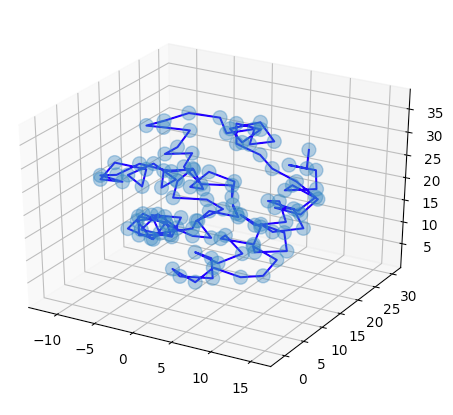
\includegraphics[width=\linewidth]{img/hom/ballRad1.png}
    \caption{A search is done near each point at increasing radii to find the nearby points }
    \label{ballRad1}
\end{figure}
The red edges indicate that the two points are less than 3.5 distance away. Making them connected.
As we increase the radius, we connect more and more points.
\begin{figure}[t]
    \includegraphics[width=\linewidth]{img/hom/ballRad2.png}
    \caption{Edges between points are formed as the search radii become larger}
    \label{ballRad2}
\end{figure}

The connections between these points form polygons (simplexes).
\begin{figure}[t]
    \includegraphics[width=\linewidth]{img/hom/ballRad3.png}
    \caption{The structure of the protein is detected as we increase the radii at around 6 Ångströms}
    \label{ballRad3}
\end{figure}
After a certain point we want to cut off our search radius because we have extracted all the notable features from our structure. If we keep increasing the search radius then all the points will be connected to each other.

A polygon is filled in when the inner polygons of the larger polygons are filled in. We note that triangles are filled as soon as they are formed but larger structures take more time to get filled in.
Persistent homology tells us when (the radius) at which these polygons are created and filled in.

Below we have two examples of the polygons.
\begin{figure}
    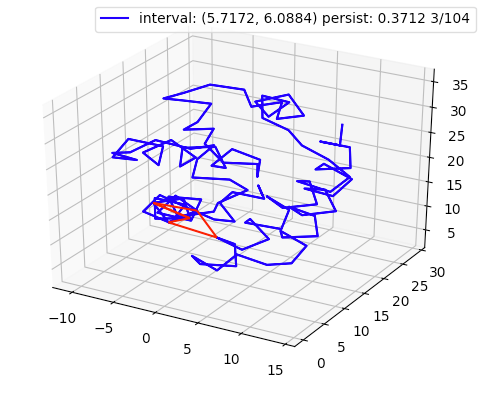
\includegraphics[width=\linewidth]{img/hom/Simplex1.png}
    \caption{Persistent Homology detecting a small cycle }
    \label{Simplex1}
\end{figure}

\begin{figure}
    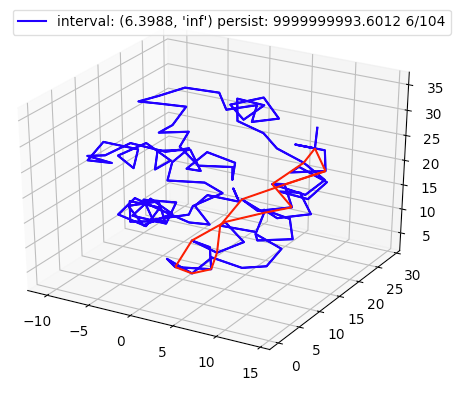
\includegraphics[width=\linewidth]{img/hom/Simplex2.png}
    \caption{Persistent homology detecting an alpha helix}
    \label{Simplex2}
\end{figure}


\begin{figure}
    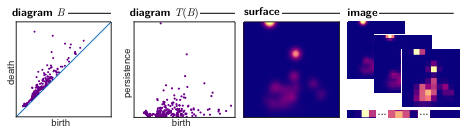
\includegraphics[width=\linewidth]{persistenceimages.png}
    \caption{For a protein, a plot of the barcodes is constructed on a 2D plane where x-coordinate is the birth and the y-coordinate is the persistence. Then, a blurred resolution of the plot is taken as the persistent image.}
    \label{persistenceimages}
\end{figure}
\subsubsection{ Sparse Persistence Homology}

\subsubsection{ Backbone Aware Persistence Homology}

\subsubsection{ Persistence Images}

The persistent homology of each protein is converted into an input feature called persistent images. For each simplex in the homology, we plot it on a 2-dimensional vector space with the x coordinate being the birth and the y coordinate being the persistence of the simplex. For the simplices that persist infinitely, we plot the y coordinates well above the maximum persistence.

This representation captures the essential information about each simplex as well as ordering them. The more persistent simplices are higher and the simplices that are born later appear towards the right.  Fig.\ref{persistencePlot} shows this plot for the protein 1ux8.

\begin{figure}
    
\includegraphics[width=\linewidth]{img/blank.png}
    \caption{Here is the plot of the simplices for the protein 1ux8. The x axis is the birth of the simplex and the y axis is the persistence of the simplex. At the very top we plot the simplices with infinite persistence.}
    \label{persistencePlot}
\end{figure}

Because it is difficult to send these pairs of points to a neural network, we take a blurred resolution of the image which is constructed as follows. First, a fixed dimensions of the blurred images is determined. Then, an interval for the x values and y values are determined experimentally by considering the intervals that contain our data. 

The plot cropped and converted to a blurred image at a set resolution. The range of the first and second coordinates to crop the plot were derived from the distribution of the data.

\begin{figure}
    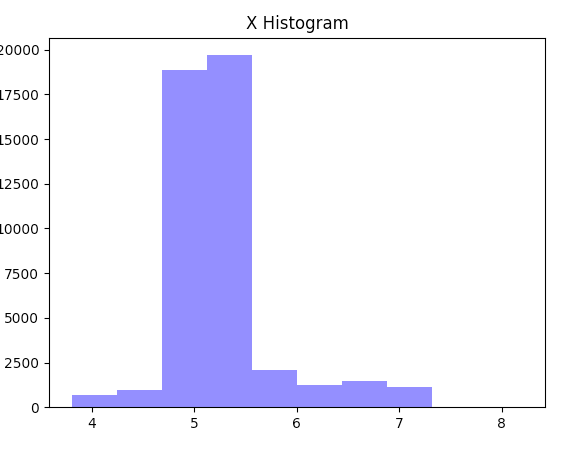
\includegraphics[width=\linewidth]{xhist.png}
    \caption{x range}
    \label{xhist}
\end{figure}

\begin{figure}
    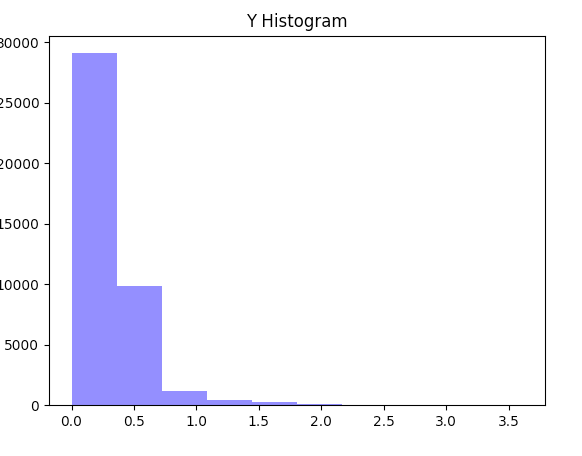
\includegraphics[width=\linewidth]{yhist.png}
    \caption{y range}
    \label{yhist}
\end{figure}


% ===============================================================
\section{Results}
% ===============================================================

%----------------------
\subsection{Distance Matrix}
%----------------------

\subsubsection{Cropped Distance Matrix}
    The distance matrix as the input feature worked pretty well for classifying the data. The best method, subsampling every other point with a window size of 50x50 gives an accuracy of 96\%
    
    The other two methods perform pretty well, at around 86\%.
    The subsampling method probably works best because it gives the neural network model to view the long range dependencies.
    The smaller window size of 50x50 performs much better than the 100x100 window for the subsampling methods.  
    
    \begin{figure}[t]
      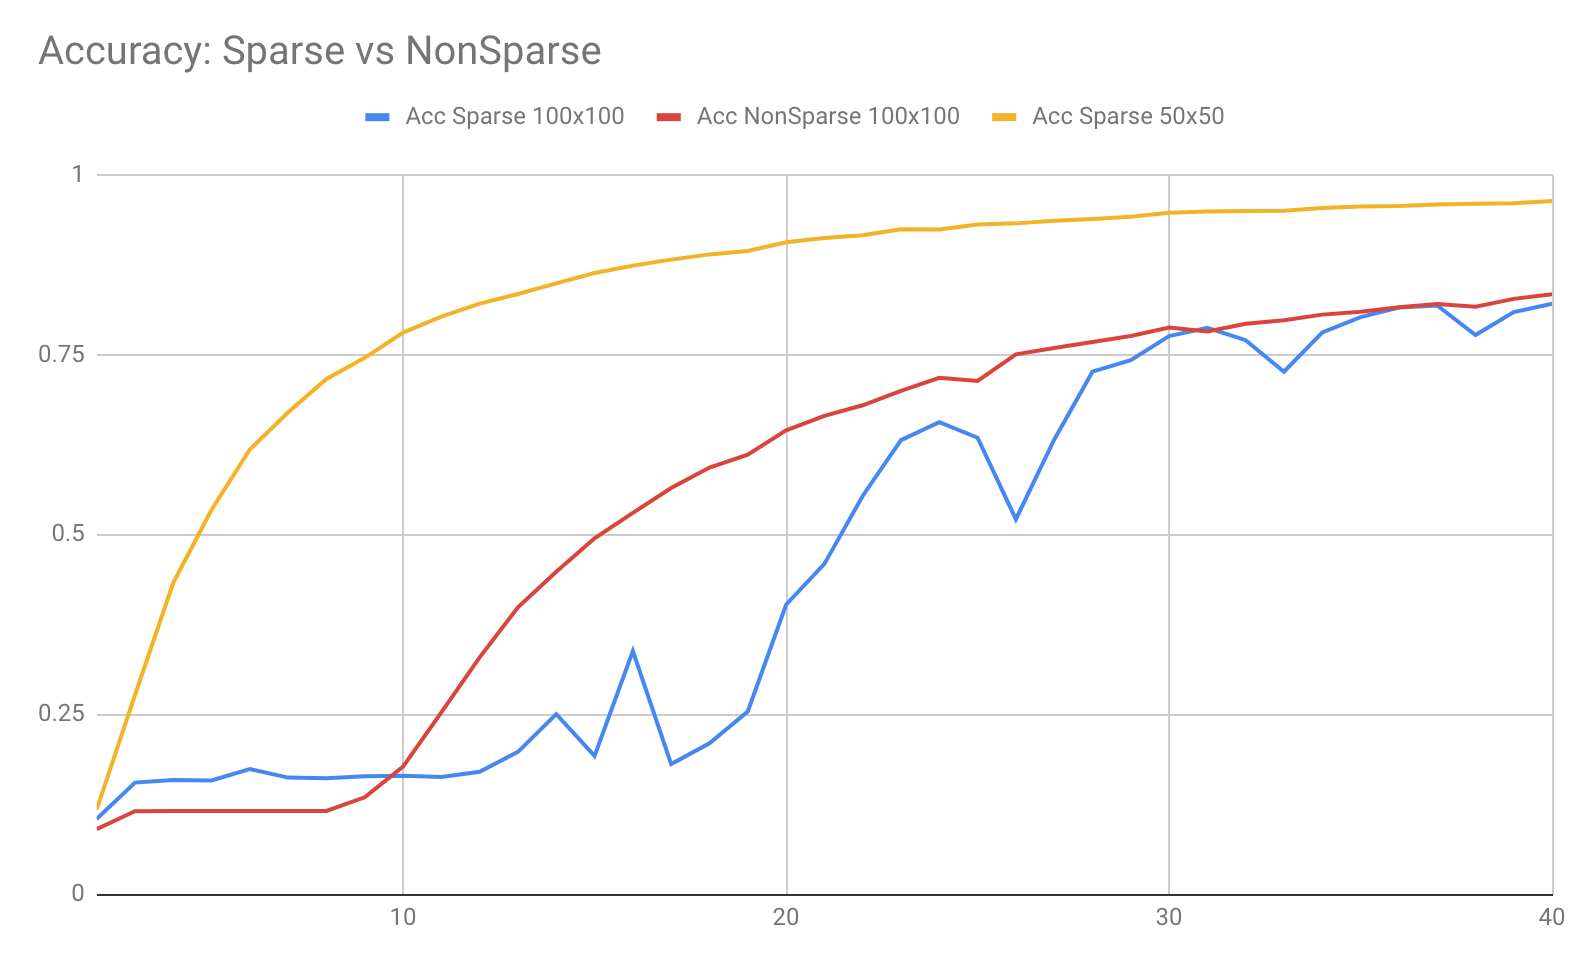
\includegraphics[width=\linewidth]{AccSparsevsNonSparse.png}
      \caption{}
      \label{AccSparsevsNonSparse}
    \end{figure}
    
    \begin{figure}[t]
      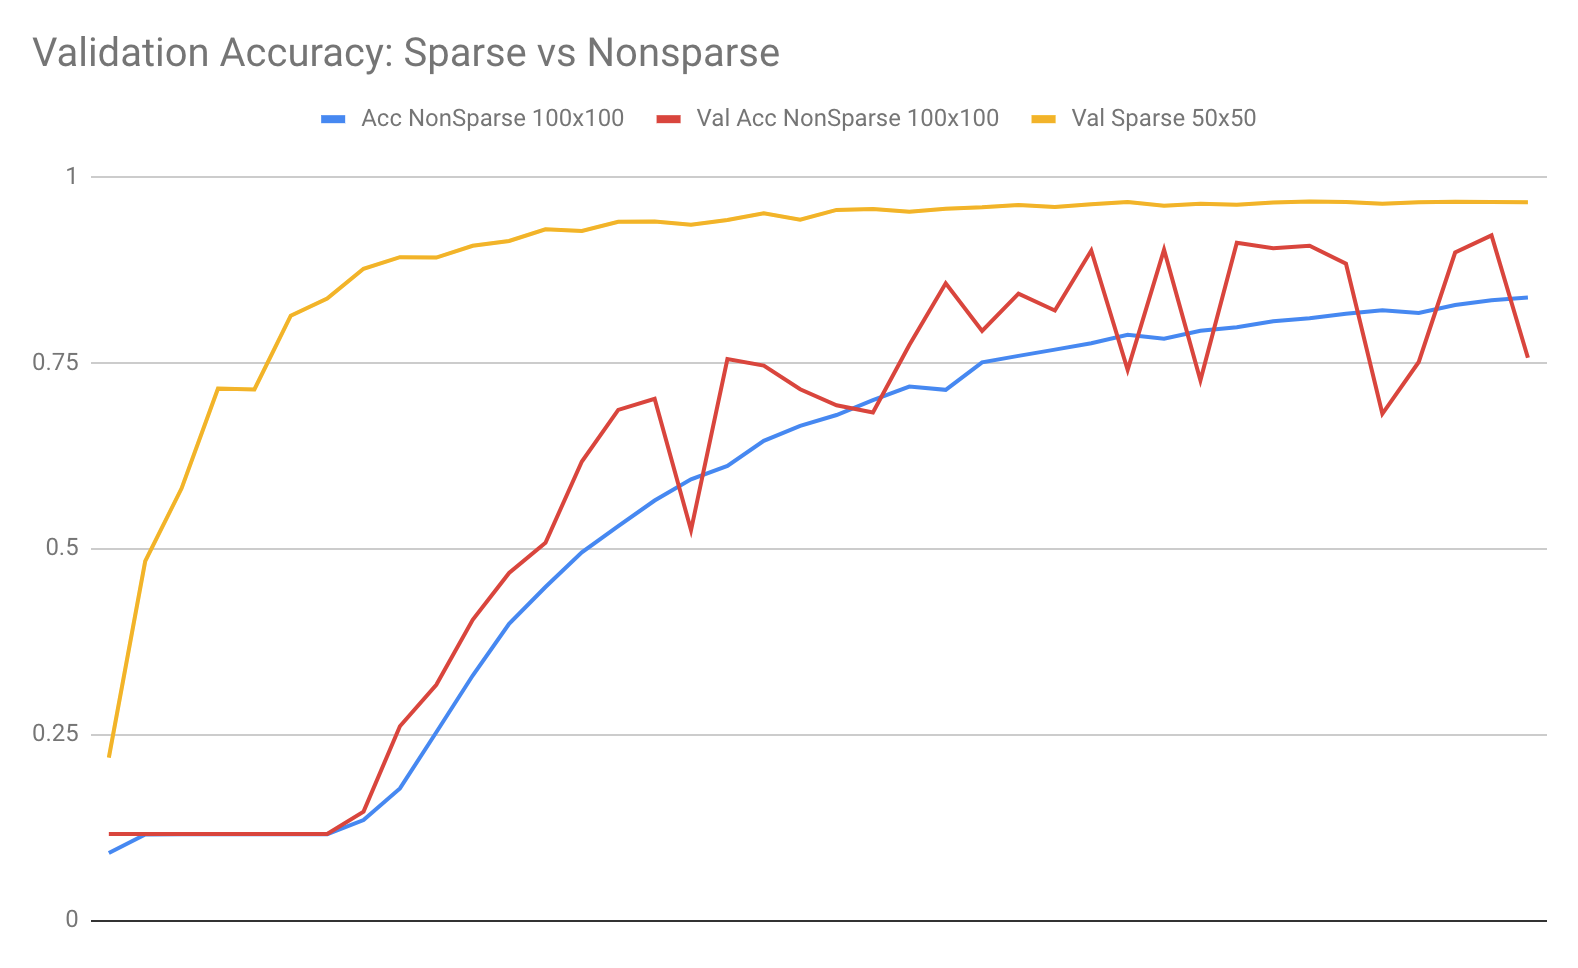
\includegraphics[width=\linewidth]{ValAccSparsevsNonsparse.png}
      \caption{}
      \label{ValAccSparsevsNonsparse}
    \end{figure}

%----------------------
\subsection{Persistent Homology}

%----------------------

%------------------------------------------------
%
%\section{Table, Figure, List Examples}
%
%\begin{figure}
%  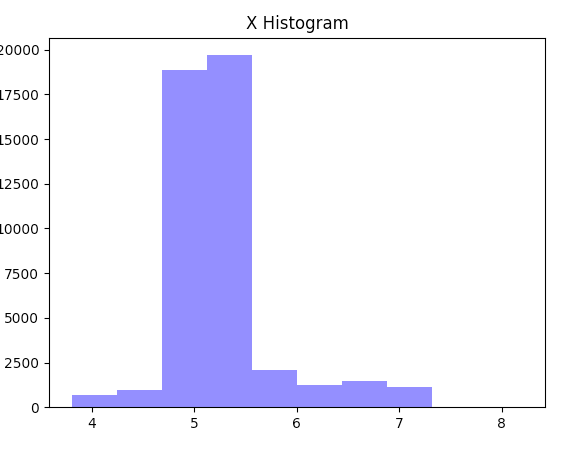
\includegraphics[width=\linewidth]{xhist.png}
%  \caption{A boat.}
%  \label{fig:boat1}
%\end{figure}
%
%\begin{table}[]
%\begin{tabular}{ccc}
%\hline
% a & a & a \\ \hline
% a & a & a \\
% a & a & a \\
% a & a & a
%\end{tabular}
%\end{table}
%
%
%\begin{itemize}
%   \item First item in a list 
%   \item Second item in a list 
%   \item Third item in a list
%\end{itemize}
%
%\begin{description}
%   \item[First] This is the first item
%   \item[Last] This is the last item
%\end{description}
%
%\begin{enumerate}
%   \item First numbered item in a list
%   \item Second numbered item in a list
%   \item Third numbered item in a list
%\end{enumerate}


%-------------------------------
%   BIBLIOGRAPHY
%---------------------------------
\pagebreak
\pagebreak
\section*{Test}
\begin{thebibliography}{9}
%APA Style
\bibitem{persistenceImages} 
Henry Adams, Tegan Emerson, and Michael Kirby. 
2017.
\textit{Persistence Images: A Stable Vector Representation of
Persistent Homology}. 
Journal of Machine Learning Research 18 (2017) 1-35

\bibitem{deepsf}
Jie Hou, Badri Adhikari and Jianlin Cheng.
2018.
\textit{DeepSF: deep convolutional neural network for mapping protein sequences to folds}
Bioinformatics, 34(8), 2018, 1295–1303

\bibitem{sakai}
Katsuro Sakai.
2010.
\textit{Simplicial Homology — A Short Course}
Institute of Mathematics University of Tsukuba

\bibitem{scope}
Fox NK, Brenner SE, Chandonia JM.
2014.
\textit{SCOPe: Structural Classification of Proteins—extended, integrating SCOP and ASTRAL data and classification of new structures.}
Nucleic Acids Research 42:D304-309. doi: 10.1093/nar/gkt1240


\bibitem{pdb}
Protein Data Bank Guide
\textit{Protein Data Bank Changes Guide
    New Changes in Version 3.20}
Nucleic Acids Research 42:D304-309. doi: 10.1093/nar/gkt1240
https://cdn.rcsb.org/wwpdb/docs/documentation/file-format/changesv3.20.pdf

\bibitem{fig:convexHull}
[Untitled illustration of convex hull]. Retrieved April 23, 2019
             from http://mathworld.wolfram.com/ConvexHull.html
             
\bibitem{fig:n-simplices}
[Untitled illustration of simplices]. Retrieved April 23, 2019
https://www.researchgate.net/figure/Simplices-from-0-simplex-to-3-simplex-11\_fig7\_290190525

\bibitem{fig:rips-complex}
[Untitled illustration of Vietoris-Rips-complex]. Retrieved April 23, 2019
https://www.researchgate.net/figure/Computation-of-PH-for-a-point-cloud-using-the-Vietoris-Rips-complex\_fig1\_279633447

\bibitem{fig:simpcomplex}
[A simplicial 3-complex]. Retrieved April 23, 2019 https://www.wikiwand.com/en/Simplicial\_complex

\end{thebibliography}

\end{document}
